\chapter{Single and multiple scattering}
\label{ch:scattering}

\section{What is computed}

The module \code{multiple_scattering.py} follows the particles one by one and \emph{counts} how many leave the sample at each scattering
angle after exactly one scattering (single) or after two or more (multiple). It works with all the geometries.

\section{Algorithm}

\begin{enumerate}
  \item Each particle starts in the beam and flies to its first interaction point in the sample (Chapter~\ref{ch:physics}).
  \item At every interaction it is \textbf{absorbed} (and lost) or \textbf{scattered}, with the probability \code{scatter_fraction} of the layer
        where it is.
  \item A scattered particle gets a new direction, drawn from the angular distribution of one scattering event, and flies on. It either interacts
        again (go to step~2) or leaves the sample.
  \item A particle that leaves the sample is counted in the bin of its final scattering angle $\twotheta$ (the angle between its final direction
        and $+z$), together with its number of scatterings.
\end{enumerate}
Particles that never interact (they miss the sample or cross it) are not scattered and are not counted. The solid angle of a bin of
$\twotheta$ between $a$ and $b$, over an azimuth range $\Delta\varphi$, is $\Delta\Omega=\Delta\varphi(\cos a-\cos b)$; dividing the counts by
the number of incident particles and by $\Delta\Omega$ gives the number of particles per incident particle per steradian, which does not depend
on the width of the bins.

\section{Calling the function}

\begin{lstlisting}
res = simulate_scattering_orders(sample, beam_width, beam_height, H=None, V=None,
                                 n_particles=200000, angle_edges_deg=None,
                                 phi_deg=0.0, phi_halfwidth_deg=None,
                                 deflection_sampler=None, max_orders=200, rng=None)
\end{lstlisting}
\begin{description}
  \item[\code{n_particles}] number of incident particles. Multiple scattering is rare, so use many (\(10^5\)--\(10^6\)).
  \item[\code{angle_edges_deg}] edges of the bins of $\twotheta$ (default: 90 bins of $2^\circ$).
  \item[\code{phi_deg}, \code{phi_halfwidth_deg}] detector window in azimuth: only the particles leaving with an azimuth within
        $\pm$\code{phi_halfwidth_deg} of \code{phi_deg} are counted. The default (\code{None}) counts all azimuths. For a detector in the horizontal plane
        (two-axis instrument) use \code{phi_deg=0} and a small half-width, which needs more particles for the same noise.
  \item[\code{deflection_sampler}] function \code{(n, rng)} returning $n$ values of $\cos\chi$ for one scattering; default isotropic;
        \code{henyey_greenstein(g)} gives a forward ($g>0$) or backward ($g<0$) peaked distribution.
\end{description}
The result \code{res} is a \code{ScatteringResult}:
\begin{center}\small
\begin{tabular}{@{}>{\raggedright\arraybackslash}p{5.6cm}p{9cm}@{}}
  \toprule \textbf{Attribute} & \textbf{Content} \\ \midrule
  \code{res.angles_deg} & bin centres of $\twotheta$ \\
  \code{res.single}, \code{res.multiple}, \code{res.total} & counts per bin of particles scattered once, two or more times, and both \\
  \code{res.counts_by_order} & table with one row for each number of scatterings (1, 2, 3, \ldots) \\
  \code{res.per_steradian(counts)} & converts counts per bin into particles per incident particle per steradian \\
  \code{res.n_incident}, \code{res.n_no_interaction}, \code{res.n_absorbed}, \code{res.n_exited} & bookkeeping: they add up to the incident number \\ \bottomrule
\end{tabular}
\end{center}
The plot is made with \code{plot_scattering_orders(res, per_steradian=True, logy=False)}.

\pyexample{ex05_scattering_orders}

\section{Results}

Figure~\ref{fig:oslab} and Figure~\ref{fig:ocyl} show the three curves for the two example samples (log scale, $10^6$ incident particles).
In the slab, $173{,}576$ of the incident particles are scattered and leave the sample: $133{,}351$ after one scattering and $40{,}225$ after two or more
(23\,\% of the scattered particles). In the cylinder, with a thicker and more attenuating inner part, $192{,}143$ leave after one scattering and
$84{,}180$ after two or more (30\,\%).

\begin{figure}[ht]
  \centering
  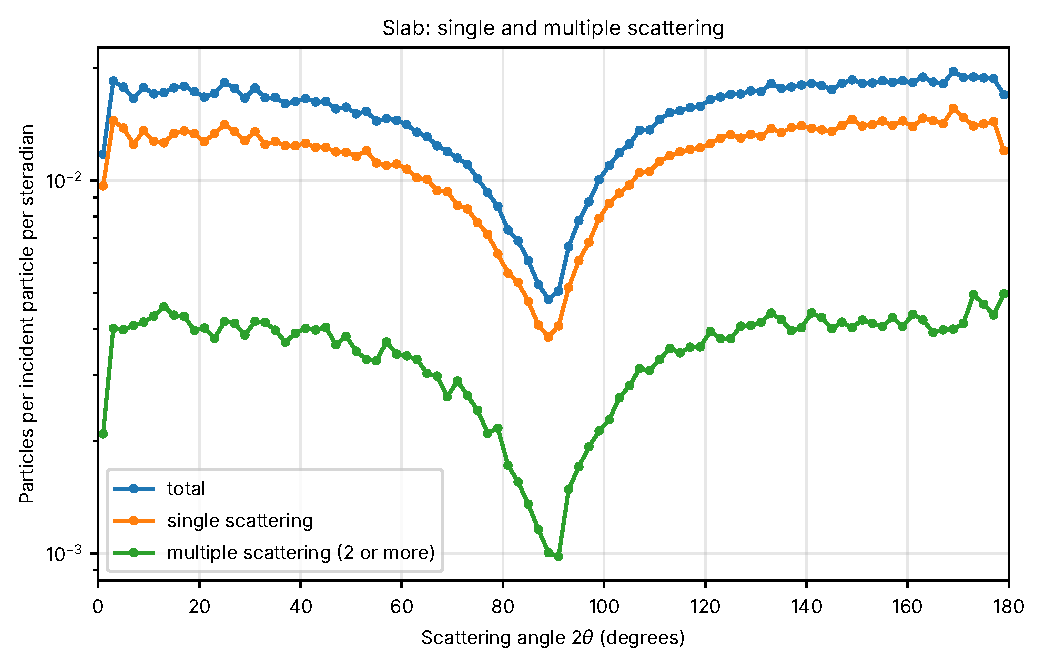
\includegraphics[width=0.8\textwidth]{fig_orders_slab}
  \caption{Slab perpendicular to the beam: total, single and multiple scattering per steradian versus $\twotheta$ ($10^6$ incident
  particles, $2^\circ$ bins). The values near $0^\circ$ and $180^\circ$ are noisy because those bins cover a very small solid angle.}
  \label{fig:oslab}
\end{figure}

\begin{figure}[ht]
  \centering
  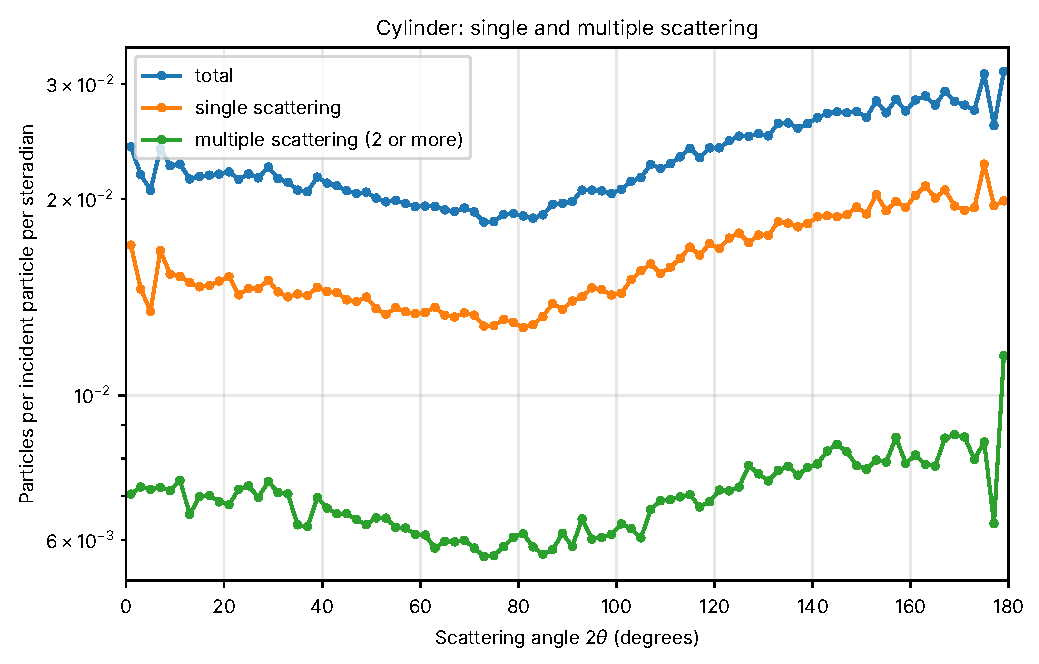
\includegraphics[width=0.8\textwidth]{fig_orders_cylinder}
  \caption{The same for the cylinder. The multiple scattering is a larger part of the total than in the slab.}
  \label{fig:ocyl}
\end{figure}

\section{Statistical error}

The number of counts in a bin follows Poisson statistics: its relative error is $1/\sqrt{N_\mathrm{bin}}$. For example, a bin with 2500 counts has an error of
2\,\%. To reduce the noise, increase \code{n_particles}, use wider bins or accept all azimuths.
